\subsection{Excercise HelloWorld}
\label{sec:excercise_hello_world}
HelloWorld is a time-honored tradition in the world of programming.
It provides a simple way to get started with a new programming language, helping to understand basic syntax and structure.
The goal of this task is to run and understand the given HelloWorld program.

This helps build a basic foundation of the Golang programming language and helps make sure the environment is set up correctly.

\subsubsection*{Run Hello World}
After following the instructions in \cite{MS-VSC}, the code is executed by running \texttt{go run main.go} in the terminal.
The code was executed twice: The first time the given code was executed leading to the output shown in \autoref{fig:screendump_helloWorld_basicExecution}.
The second time the code was executed with different text, which can be seen in \autoref{fig:screendump_helloWorld_differentText}.

\begin{figure}[H]
    \centering
    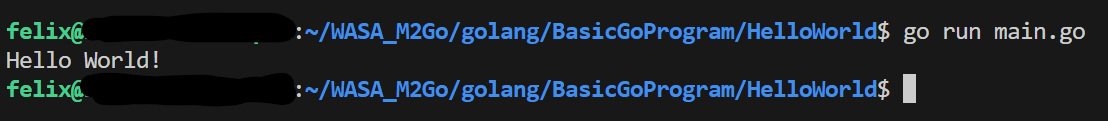
\includegraphics[width=0.8\textwidth]{figures/goLang/helloWorld/golang_helloWorld_basicExecution.png}
    \caption{Screendump showing the Basic Execution of the Hello World Program}
    \label{fig:screendump_helloWorld_basicExecution}
\end{figure}

\begin{figure}[H]
    \centering
    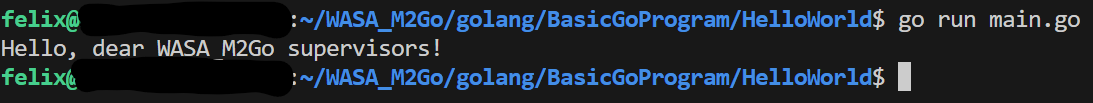
\includegraphics[width=0.8\textwidth]{figures/goLang/helloWorld/golang_helloWorld_ExecutionDifferentText.png}
    \caption{Screendump showing the Execution of the Hello World Program with altered Output}
    \label{fig:screendump_helloWorld_differentText}
\end{figure}

\subsubsection*{Explain HelloWorld}
\autoref{lst:helloWorld} shows the code of the Hello World program with explanations of the different parts of the code.
\begin{lstlisting}[
style=kit-cm,
language=Golang,
caption={Hello World Program in Golang with Explanations},
label={lst:helloWorld},
]
// main.go 
// Author: Felix Weik

package main    // package declaration: every executable belongs to the main package
                // by declaring this package, an executable file is produced after compilation

import "fmt"    // import the fmt package, a standard library package 
                // implementing formatted I/O functions
                // after import, one can use the functions of the imported package

func main() {   // declares the function main, which is the 
                // entry point of the program
    fmt.Println("Hello, World!")    // call the Println function 
                                    // of the fmt package; Println prints 
                                    // the given text to the standard output
}               // end of the main function

\end{lstlisting}

\subsubsection*{Extend HelloWorld}
The goal of this task is to extend the already given HelloWorld program to the HelloName program, prompting the user for a name and then showing the given prompt in the output.
The code is shown in \autoref{lst:helloName}:
\begin{lstlisting}[
style=kit-cm,
language=Golang,
caption={Extension of helloWorld to helloName},
label={lst:helloName},
]
// main.go
// Author: Felix Weik

package main

import (
    "fmt"
)

func main() {
    greet()
}

func greet() {
    var name string
    fmt.Print("What is your name? ")
    fmt.Scanln(&name)
    fmt.Println("Hello, " + name + "!")
} 
\end{lstlisting}

The result of the executed code is shown in \autoref{fig:screendump_helloName}

\begin{figure}[H]
    \centering
    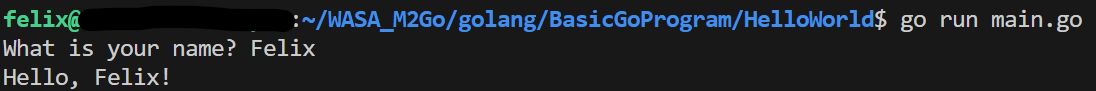
\includegraphics[width=0.8\textwidth]{figures/goLang/helloWorld/golang_helloWorld_helloName.png}
    \caption{Screendump showing \texttt{HelloName}'s Execution}
    \label{fig:screendump_helloName}
\end{figure}